\section{Malware Information Retrieval System}
% 목표하는 바
이번 세션에서는 제안된 malware information retrieval system 의 동작과 구성 그리고 가져야하는 속성들을 설명한다. 우리의 시스템은 크게 학습과 검색(retrieval), 두 페이즈로 나뉜다. 학습 페이즈에서는 원할한 검색을 위해 시멘틱스를 반영하는 학습 데이터의 표현 벡터를 학습한다. 검색 페이즈에서는 유저로부터 입력된 멀웨어 혹은 태그 쿼리와 미리 저장해놓은, 학습된 표현 벡터들로부터 랭킹 결과를 출력한다. 이어지는 서브 섹션에서는 두 페이즈에서 사용될 노테이션들을 정의하고, 이들을 이용해서 각 페이즈에서 어떤 태스크를 행해야하는지를 자세히 설명한다.  


\subsection{Notations}
우리는 먼저 학습 멀웨어 셋으로 $X = \{x_1, x_2, ..., x_N\}$ 를 갖고있다. 그리고 각 멀웨어에 해당하는 싱글레이블 셋 $Y_s = \{y_{s1}, y_{s2}, ..., y_{sN}\}$ 과 멀티레이블 셋 $Y_m = \{\vec{y}_{m1}, \vec{y}_{m2}, ... , \vec{y}_{mN}\}$ 이 있다. 이 레이블을 얻는 방법은 섹션 6.1에서 설명한다. 그리고 각 멀웨어로부터 손으로 추출된 피쳐들의 셋을 $V = \{v_1, v_2, ..., v_n \}$ 로 정의한다. 

멀웨어 IR 시스템은 $[h, E, d, R]$ 4개의 원소를 갖는 tuple 로 정의된다. $h$ 는 멀웨어 피쳐로부터 벡터 representation 을 얻을 수 있는 임베더 함수이다. $E$ 는 검색이 될 멀웨어의 임베딩 벡터 셋이다. $d$ 는 입력된 쿼리와 임베딩 벡터 간 거리를 계산하는 함수이다. $R$ 은 랭킹 모듈이다. 학습 페이즈에서는 적절한 $h$ 를 학습하고 이를 통해 $V$로부터 $E$를 얻는다. 리트리벌 페이즈에서는 멀웨어 샘플 쿼리 $q$ 를 입력받고 가장 가까운 $k$ 개의 neighbor 를 랭킹 모듈 $R$ 을 통해 반환한다.

\begin{table}[!htb] % notation
\caption{Notations}
\label{tab:notation}
\begin{minipage}{\columnwidth}
\begin{center}
\begin{tabular}{ll}
\toprule
Meaning & Notation\\
\midrule
  Set of malwares     & $X$ \\
  ith malware sample  & $x_i$ \\
  Set of single labels & $Y_s$ \\
  Single label of ith malware    & $y_{si}$ \\
  Extracted features of ith malware & $v_i$ \\
  Set of extracted features   & $V$ \\
  Set of multilabels   & $Y_m$ \\
  Multilabels of ith malware & $\vec{y}_{mi}$\\
  Neural embedder & $h$ \\
  Parameters of neural embedder & $\theta$ \\
  Classifier & $g$ \\   
  Parameters of classifier & $W$, $b$ \\  
  Set of Embedded malware vectors & $E$ \\
  Embedded malware vector & $e$ \\
  Importance coefficient & $c$ \\
  Distance measuring function & $d$ \\
  Semantic component vector & $s$ \\
  Ranking Module & $R$\\
\bottomrule
\end{tabular}
\end{center}
\bigskip\centering
\end{minipage}
\end{table}


\subsection{Tasks}
학습페이즈에서는 IR system 에서 사용하기 위한 벡터 리프레젠테이션을 얻기 위한 Auxiliary Task를 수행한다. Auxiliary Task 는 멀웨어 분류 태스크를 학습하는 것으로 싱글 레이블 클래시피케이션이나 멀티레이블 클래시피케이션이 될 수 있다. $f: V \rightarrow Y $ 인 f 는 멀웨어 피쳐로부터 레이블을 추정하는 함수이다. 함수 $f$ 는 다시 $g$ 와 $h$ 의 합성 함수로 정의할 수 있다. $h$ 는 위에서 설명한, 멀웨어 피쳐로부터 vector representation 을 얻을 수 있는 임베딩 함수이다. $g$는 임베딩으로부터 label 을 추정할 수 있는 클래시파이어이다. 시멘틱을 내포하는 임베딩 벡터를 학습시키는 방법에 대해서는 섹션4에서 자세히 이야기한다. 
\[
f(v_i) = (g \circ h)(v_i) = g(h(v_i)) = g(e_i) = y_i 
\]
where
\[
g(e_i) = \sigma (W*e_i + b) 
\]
% sigma == sigmoid or softmax
리트리벌 페이즈에서는 멀웨어 샘플 쿼리 q를 입력받아 학습 페이즈에서 구했던 h 함수를 이용하여 임베딩한다. 임베딩된 쿼리 eq 와 E 의 원소들 간 거리를 d 함수를 통해 측정하고, 가까운 k 개의 neighbor 를 랭킹 모듈 R 을 통해 반환한다. 

% Algorithm 으로 대체
\[
Results = \{x_j | j = argmin_i( {-d(e_q, e_i)} )  \}
\]


\subsection{Modules}
두 페이즈의 구조도는 Figure 과 같다. 두 페이즈에서 공통으로 존재하는 모듈은 Feature Extractor와 Neural Embedder 가 있다. 벡터 학습 페이즈에는 Classifier 가, 리트리벌 페이즈에는 랭킹 모듈이 포함되어있다. 

\begin{figure}[!htb] % train_phase
  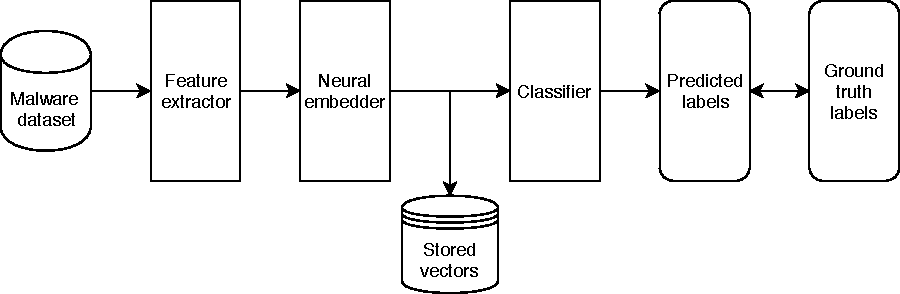
\includegraphics[width=\linewidth]{../figures/train_phase.pdf}
  \caption{train phase}
  \label{fig:train_phase}
\end{figure}

\begin{figure}[!htb] % retrieval_phase
  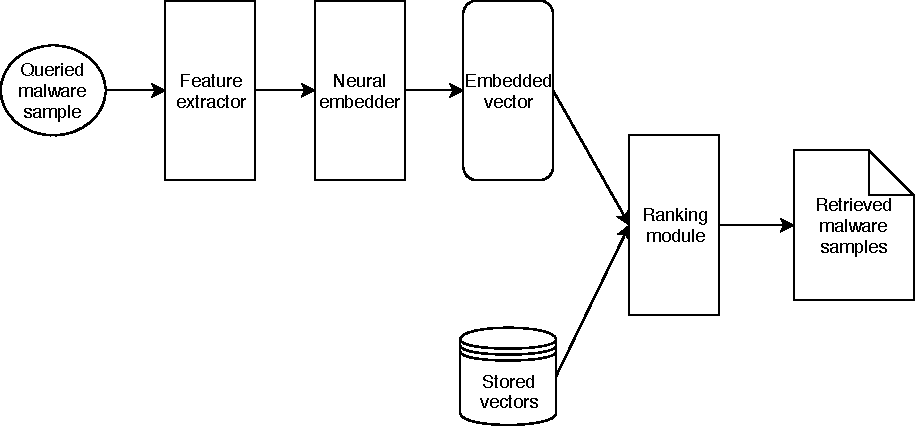
\includegraphics[width=\linewidth]{../figures/retrieval_phase.pdf}
  \caption{retrieval phase}
  \label{fig:retrieval_phase}
\end{figure}

\textbf{Feature Extractor. }
Feature extractor 는 Malware Rawdata 로부터 Handcrafted feature 를 추출하는 모듈이다. Handcrafted feature로 PE 같은경우에는 Size 와 Entropy, Histogram of API Calls, … 등을[*] 추출한다. APK 같은 경우에는 추가적으로 Permission,  … 등의 피쳐를 추출한다. 

\textbf{Neural Embedder. }
Neural embedder 는 Feature extractor 모듈에서 추출된 멀웨어의 피쳐들로부터 Representation vector 를 뽑는 모듈이다. theta 로 Parameterized 되어있는 뉴럴 네트워크이며, 파라미터는 벡터 학습 페이즈에서 Auxiliary Task 를 수행하면서 Optimize 된다. 그리고 리트리벌 페이즈에서 파라미터는 freeze 되어 업데이트되지 않는다. 
Neural Embeder 의 네트워크 구조는 CNN을 사용하였다. Thumbnail 을 받아서 CNN 5 층과 fully 2 층을 쌓은 구조를 사용한다. feature 의 성격에 따라 다른 네트워크 구조로 임베딩 피쳐벡터를 추출함으로써 더 나은 generalization 성능을 얻을 수 있다. thumbnail 피쳐는 [malimg 논문 인용] 악성 코드영역 혹은 악성코드를 특징짓는 영역의 로컬리 시프트 인베리언트한 특성을 담기 위해 CNN 을 사용해서 임베딩 피쳐벡터를 추출한다. 

\textbf{Classifier. }
%% Figure
%\begin{figure}
%  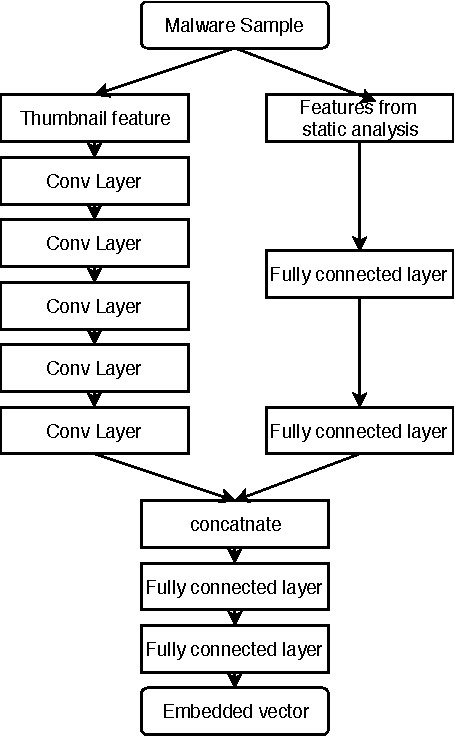
\includegraphics[height=10cm]{../figures/neural_embedder.pdf}
%  \caption{neural embedder}
%  \label{fig:three}
%\end{figure}
Classifier 모듈은 Neural embedder 를 통과해서 나온 embedding vector 를 받아서 각 레이블 별 확률을 출력해준다. 1층의 fully connected 로 파라미터라이즈드 되어있으며 태스크에 따라 softmax 혹은 sigmoid Activation을 사용하였다. Neural Embeder 모듈과 마찬가지로 벡터 학습 페이즈에서 back propagation 에 의해 파라미터들이 학습되고, 리트리벌 페이즈에서는 프리즈된다. 

\textbf{Ranking Module. }
학습 페이즈에 저장해두었던 학습 셋의 임베딩 벡터들과 추출된 벡터의 거리를 거리함수 d 를 사용하여 측정하고 k 개의 nearest neighborhood 를 가까운 순서대로 정렬하고 출력한다.


\subsection{Desired properties}
멀웨어 IR 시스템은 한계들이 존재했다. 특히 Raw binary file 로부터 좋은 피쳐를 뽑기가 수월하지 않고, intraclass variance 는 크고 innerclass variance 는 작으며 계속해서 변종과 새로운 종이 생겨나는 멀웨어 도메인의 특징으로 말미암아 좋은 멀웨어 IR 시스템이 가져야 할 속성들은 다른 도메인의 IR 시스템과는 조금 다르다.

\textbf{Semantic understanding. }
쿼링 샘플에 대해 구조적으로 비슷한 샘플 뿐만 아니라 의미적으로도 비슷한 샘플들을 랭킹하고 retrieve 할 수 있어야 한다. 여기서 의미가 비슷하는 것은 멀웨어의 행동 혹은 사람이 생각하기에 중요한 멀웨어의 속성들이 비슷하다는 것을 의미한다. 구조적으로 다르다고 해도 멀웨어의 행위가 일치하면 같은 의미를 갖는 샘플이라고 볼 수 있다. 마찬가지로 구조적으로 거의 같다고 해도 멀웨어의 행위가 전혀 다르다면 두 샘플은 다른 의미를 가졌다고 할 수 있다. 더불어 우리는 Locky 와 Cerber 라는 두 랜섬웨어 패밀리에 해당하는 샘플 간 유사도가 Locky 와 Coinminer 에 해당하는 두 샘플의 유사도보다 더 작다고 생각한다. 이러한 샘플들 간 의미 차이 까지 고려될 수 있다면 그 시스템은 Symantics-aware한 시스템이라고 할 수 있다. 
 
\textbf{Robustness to novel samples. }
멀웨어의 새로운 변종들은 계속해서 나타나기 때문에 이에 빠르게 대응할 수 있어야 한다. 
%
%\textbf{Robustness to rare inputs. }
%멀웨어 도메인에서의 샘플 수는 그 멀웨어 패밀리의 영향력을 의미하지 않는다. 물론 비례하는 경향이 없는것은 아니지만, 하나의 멀웨어가 전세계적으로 유행할 수도 있고, 변종은 많지만 별로 영향력이 없는 멀웨어일 수도 있다. 따라서 해당 패밀리의 샘플 수가 적다고해서 쿼링 결과에서 랭킹 순위가 밀려서는 안된다. 즉 적은 수의 샘플에 대해서도 모델은 강건해야한다. 

%\textbf{Robustness to variable size inputs. }
%멀웨어의 raw file size Variance 는 매우 크다. 작게는 몇키로바이트부터 크게는 기가단위까지 갈 수 있다. 사이즈에 상관없이 retrieve 를 할 수 있어야 한다.

\textbf{Efficiency. }
세상에 존재하는 멀웨어 샘플 개수는 매우 많고 기하급수적으로 늘어나고 있다. 따라서 수많은 샘플들에서 k 개의 상위 랭크된 결과를 적절한 시간 내에 retrieve 하려면 랭킹 모듈이 효율적이어야한다.



